
\section{Google Chromecast}

%-----------------------    ---------------------------------

\begin{frame}
\frametitle{Google Chromecast}

\begin{center}
  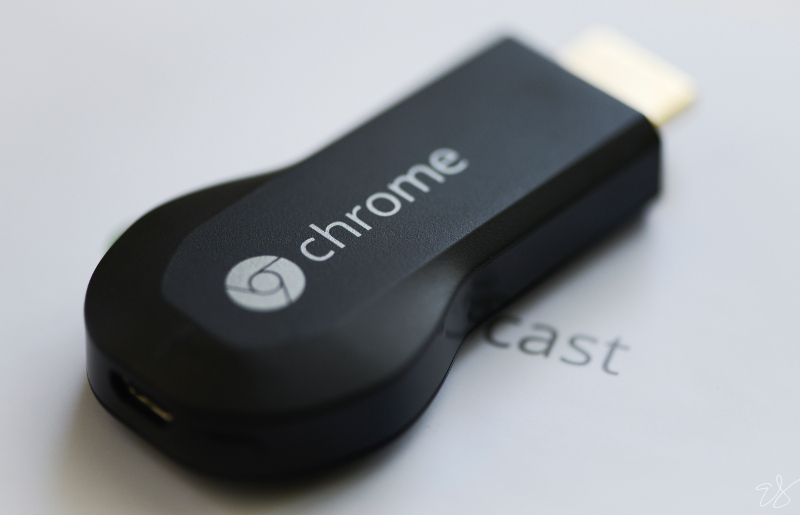
\includegraphics[width=10cm]{figs/chromecast.jpg}
\end{center}


\begin{flushright}
{\tiny
Source: Wikipedia
}
\end{flushright}

\end{frame}



%-----------------------    ---------------------------------

\begin{frame}
\frametitle{Google Chromecast conectado}

\begin{center}
  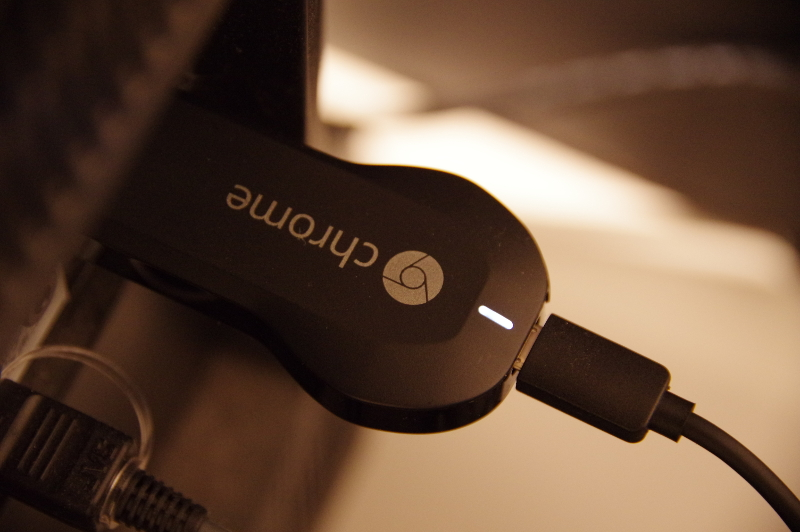
\includegraphics[width=10cm]{figs/enlatele.jpg}
\end{center}


\begin{flushright}
{\tiny
Source: Wikipedia
}
\end{flushright}

\end{frame}



%-----------------------    ---------------------------------

\begin{frame}
\frametitle{¿Qué es Chromecast?}

\begin{itemize}
   \item Permite convertir tu TV en un \emph{smart TV}
   \item Se maneja desde un dispositivo móvil
   \item Las aplicaciones pueden tener soporte para Chromecast
   \item Se conecta al puerto HDMI de la TV y la wifi
   \item Permite hacer \emph{streaming}
   \item Cuesta 35 euros
   \item Programable mediante SDK propio
\end{itemize}

\end{frame}


%-----------------------    ---------------------------------

\begin{frame}
\frametitle{Tu móvil en la TV}

\begin{center}
  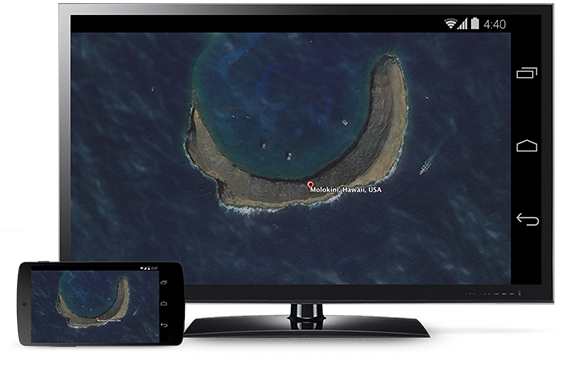
\includegraphics[width=10cm]{figs/mirror.png}
\end{center}


\begin{flushright}
{\tiny
Source: Google
}
\end{flushright}

\end{frame}


